\chapter{Desarrollo del proyecto}
\label{cap:estadodelarte}


\section{Antecedentes de la empresa}

\subsection{Descripción de la empresa}

3Dlux es un emprendimiento dedicado al diseño e impresión 3D, fundada el año 2016 por Javier Oliva y Juan Marinetti. La empresa comenzó con el propósito de utilizar la tecnología de impresión 3D FDM para la fabricación de piezas, enfocadas principalmente a las soluciones del área industrial y manufactura. Así, el año 2017 la empresa comenzó con una etapa de investigación y aprendizaje de la maquinaria para estos efectos, y la posibles industrias en las cuales la impresión 3D podría agregar valor. El interés de Javier, diseñador de profesión, por trabajar con softwares de diseño 3D y la visión de Juan, empresario, por incursionar en nuevas áreas de negocio, fueron dando forma al estado actual de la empresa. 
La primera capacitación o acercamiento a la industria fue en Estados Unidos, donde Javier estuvo de pasante en la empresa de impresión 3D \textit{3DChimera} durante dos semanas. Tanto las máquinas como el modelo de negocio que utilizaban, fueron tomados como ejemplo para lo que se implementaría en Chile. Posterior a este hecho, el primer año de desarrollo se llevó a cabo con la colaboración de la empresa \textit{Acrus-ccl}, dedicada al etiquetado de vinos ubicada en la comuna de Conchalí. Allí, haciendo uso de una oficina facilitada para estos efectos, se instalaron las primeras máquinas e impresoras 3d, haciendo trabajos ocasionales y a pedido. En 2018, la empresa se trasladó a las dependencias de la Fundacion Mustakis, en la comuna de Recoleta, emplazamiento que ocupa en la actualidad. Hoy, el taller cuenta con 9 impresoras 3d y desarrolla piezas para distintas industrias como minería, salud, entre otras. La capacidad instalada ha permitido la producción de piezas de un volumen aproximado de 300 unidades por pedido; asimismo, la diversidad de impresoras da la posibilidad de trabajar con diversos filamentos de impresión 3D, tanto materiales tradicionales (PLA, ABS y PETG) como plásticos de ingeniería (ASA, PC, entre otros). Dentro de los servicios ofrecidos está el diseño y fabricación de productos y piezas, escaneo 3D y capacitaciones orientadas al uso de las máquinas. 




\section{Descripción del Problema}

Las ventajas del proceso de impresión 3D FDM como la fabricación de diseños complejos, el bajo coste de inversión y la obtención de un objeto final, han hecho que muchas empresas dedicadas al rubro de la manufactura comiencen a incorporar a sus lineas estas máquinas. Por otra parte, la existencia de pequeñas empresas y emprendimientos dedicados a la impresión 3D ha generado un avance en el conocimiento, aplicación y difusión de esta tecnología. Sumado a lo anterior, la personalización de los productos en masa da lugar a que, para maximizar la producción, es necesario el control y la gestión de una mayor cantidad de impresoras. Es por esto que, a mayor cantidad de máquinas, también aumenta la complejidad, ya sea en la operación misma, o mantenerlas en un estado confiable y disponible. A medida que fue aumentando la cantidad de activos, la empresa se vio en la necesidad de optimizar el proceso de producción y mantenimiento, detectando los siguientes problemas:

\begin{itemize}
\item Imposibilidad de monitorización de múltiples máquinas funcionando a la vez.
\item Impresoras detenidas frecuentemente por mantenimiento correctivo.
\item Impresoras detenidas por varias horas debido a dificultades con la identificación de los problemas.
\item Existencia nula o insuficiente de datos referidos a los mantenimientos realizados.
\item Existencia nula o insuficiente de datos referidos al material utilizado.
\end{itemize}





\section{ Aplicación de mantenimiento basado en la teoría de la confiabilidad}


\subsection{Selección del equipo}

\subsubsection{Análisis de criticidad}

El primer paso para determinar la máquina de impresión 3D más crítica, es la realización de un análisis de criticidad a los equipos del taller. Debido a que la empresa no ha registrado periódicamente las fallas ocurridas y las acciones de mantenimiento realizadas, el análisis se basará en establecer cual sería la condición más favorable, así como la condición menos favorable de cada uno de los criterios a evaluar, según apreciaciones generales e información obtenida en los últimos seis meses. Para esto, los aspectos a evaluar son:

\begin{itemize}
\item Impacto a la seguridad
\item Costo de reparación
\item Frecuencia de las fallas
\item Costo operacional
\end{itemize}

Las tablas de ponderaciones para cada uno de estos son las siguientes:

\begin{table}[H]
  \centering
  
    \begin{tabular}{|l|r|}
    \hline
    Frecuencia de las fallas & \multicolumn{1}{l|}{Ponderación} \\
    \hline
    mayor que 16 /semestre & 5 \\
    \hline
    12-15/semestre & 4 \\
    \hline
    8-11/semestre & 3 \\
    \hline
    4-7/semestre & 2 \\
    \hline
    Menor a 4/al semestre & 1 \\
    \hline
    \end{tabular}%
    \caption{Ponderaciones para el ítem de frecuencia de fallas}
  \label{tab:addlabel}%
\end{table}%

\qquad\qquad%

\begin{table}[H]
  \centering
 
    \begin{tabular}{|l|r|}
    \hline
    Costo de reparación & \multicolumn{1}{l|}{Ponderación} \\
    \hline
    mayor a \$80.000 & 10 \\
    \hline
    \$60.000 - \$79.000 & 8 \\
    \hline
    \$40.000 - \$59.000 & 6 \\
    \hline
    \$20.000 - \$39.000 & 4 \\
    \hline
    Menor a \$20.000 & 2 \\
    \hline
    \end{tabular}%
    \caption{Ponderaciones para el ítem de costo de reparación}
  \label{tab:addlabel}%
\end{table}%

\begin{table}[H]
  \centering
 
    \begin{tabular}{|l|r|}
    \hline
    Impacto a la seguridad & \multicolumn{1}{l|}{Ponderación} \\
    \hline
    Muy grave & 10 \\
    \hline
    Grave & 8 \\
    \hline
    Severo  & 6 \\
    \hline
    Moderado & 4 \\
    \hline
    Bajo  & 2 \\
    \hline
    \end{tabular}%
    \caption{Ponderaciones para el ítem de Impacto a la seguridad}
  \label{tab:addlabel}%
\end{table}%

\begin{table}[H]
  \centering
  
    \begin{tabular}{|l|r|}
    \hline
    Impacto Operacional & \multicolumn{1}{l|}{Ponderación } \\
    \hline
    Para la operación & 15 \\
    \hline
    80\% de parada & 12 \\
    \hline
    60\% de parada & 9 \\
    \hline
    40\% de parada & 6 \\
    \hline
    20\% de parada & 3 \\
    \hline
    \end{tabular}%
    \caption{Ponderaciones para el ítem de impacto operacional}
  \label{tab:addlabel}%
\end{table}%

Los resultados del análisis de criticidad para elegir el activo más crítico se muestran en la siguiente tabla:

\begin{table}[H]
  \centering
  
    \scalebox{0.75}{\begin{tabular}{|r|l|l|l|l|l|l|l|}
    \hline
    \multicolumn{1}{|l|}{Ítem} & Activo & \multicolumn{1}{p{2cm}|}{Frecuencia de fallas} & \multicolumn{1}{p{2cm}|}{Seguridad} & \multicolumn{1}{p{2cm}|}{Operacional} & \multicolumn{1}{p{2cm}|}{Reparación} & \multicolumn{1}{p{1cm}|}{Total Consec.} & \multicolumn{1}{p{1cm}|}{Critic. Total} \\
    \hline
    1     & Impresora PRUSA MK3 & 1 & 2& 9 & 8& 19& 19 \\
    \hline
    2     & Impresora ENDER 3 & 1  & 2 & 6 & 4 & 12 & 12 \\
    \hline
    3     & Impresora X350 G. RepRap & 3& 4 & 12 & 8  & 24 & 72 \\
    \hline
    4     & Impresora X400 G. RepRap & 2 & 4 & 12 & 8 & 24 & 48 \\
    \hline
    \end{tabular}}
    \caption{Análisis de criticidad para determinar el activo más crítico.}
  \label{tab:addlabel}%
\end{table}%

El puntaje final se obtiene multiplicando el valor obtenido de las frecuencias por la sumatoria total de las consecuencias para cada Activo. De este análisis se desprende que la impresora \textit{X350 German RepRap} es el equipo con mayor criticidad en función de las variables estudiadas, en el periodo comprendido por seis meses desde marzo hasta agosto del 2020.

\subsection{Descripción del equipo}

La máquina modelo X350 de la fundación GermanRepRap es una impresora 3D de código abierto, dirigida tanto a consumidores en general como a usuarios industriales. Posee un cabezal de doble extrusión, superficie de construcción rectangular descendente con respecto al eje-z y  climatizada. El volumen total de la máquina es de 600x444x517 mm y el volumen de construcción comprende los 350x200x210 mm.

A continuación, se resumen los datos técnicos generales de la máquina: 

\begin{table}[H]
  \centering
  
    \begin{tabular}{|l|l|}
    \hline
    Materiales & ABS, PLA, PS, PP, PVA \\
    \hline
    Dimensiones & 600x444x517 mm \\
    \hline
    Volumen de impresión & 350x200x210 mm \\
    \hline
    Voltaje de Operación & 110/230 V \\
    \hline
    Consumo & 250 W \\
    \hline
    Configuración  & Unidad prefabricada/Lista para imprimir \\
    \hline
    Tecnología & FDM \\
    \hline
    Grosor de capa & 0,02 mm \\
    \hline
    Velocidad de impresión  & 10-150 mm/s \\
    \hline
    Velocidad de viaje & 10-300 mm/s \\
    \hline
    Cama de impresión & T° max 120°C \\
    \hline
    Conexión a red & WLAN/Ethernet \\
    \hline
    Peso  & 29 Kg \\
    \hline
    Boquilla & 0,4 mm \\
    \hline
    \end{tabular}%
    \caption{Ficha Técnica de la máquina X350 German RepRap \citep{germanreprap2019}.}
  \label{tab:addlabel}%
\end{table}%



\begin{table}[H]
\centering
\begin{tabular}{p{6cm}p{6cm}}
\includegraphics[scale=0.04]{images/x350front.jpg} & \includegraphics[scale=0.04]{images/x350inf.jpg}\\
\includegraphics[scale=0.04]{images/x350lat.jpg} & 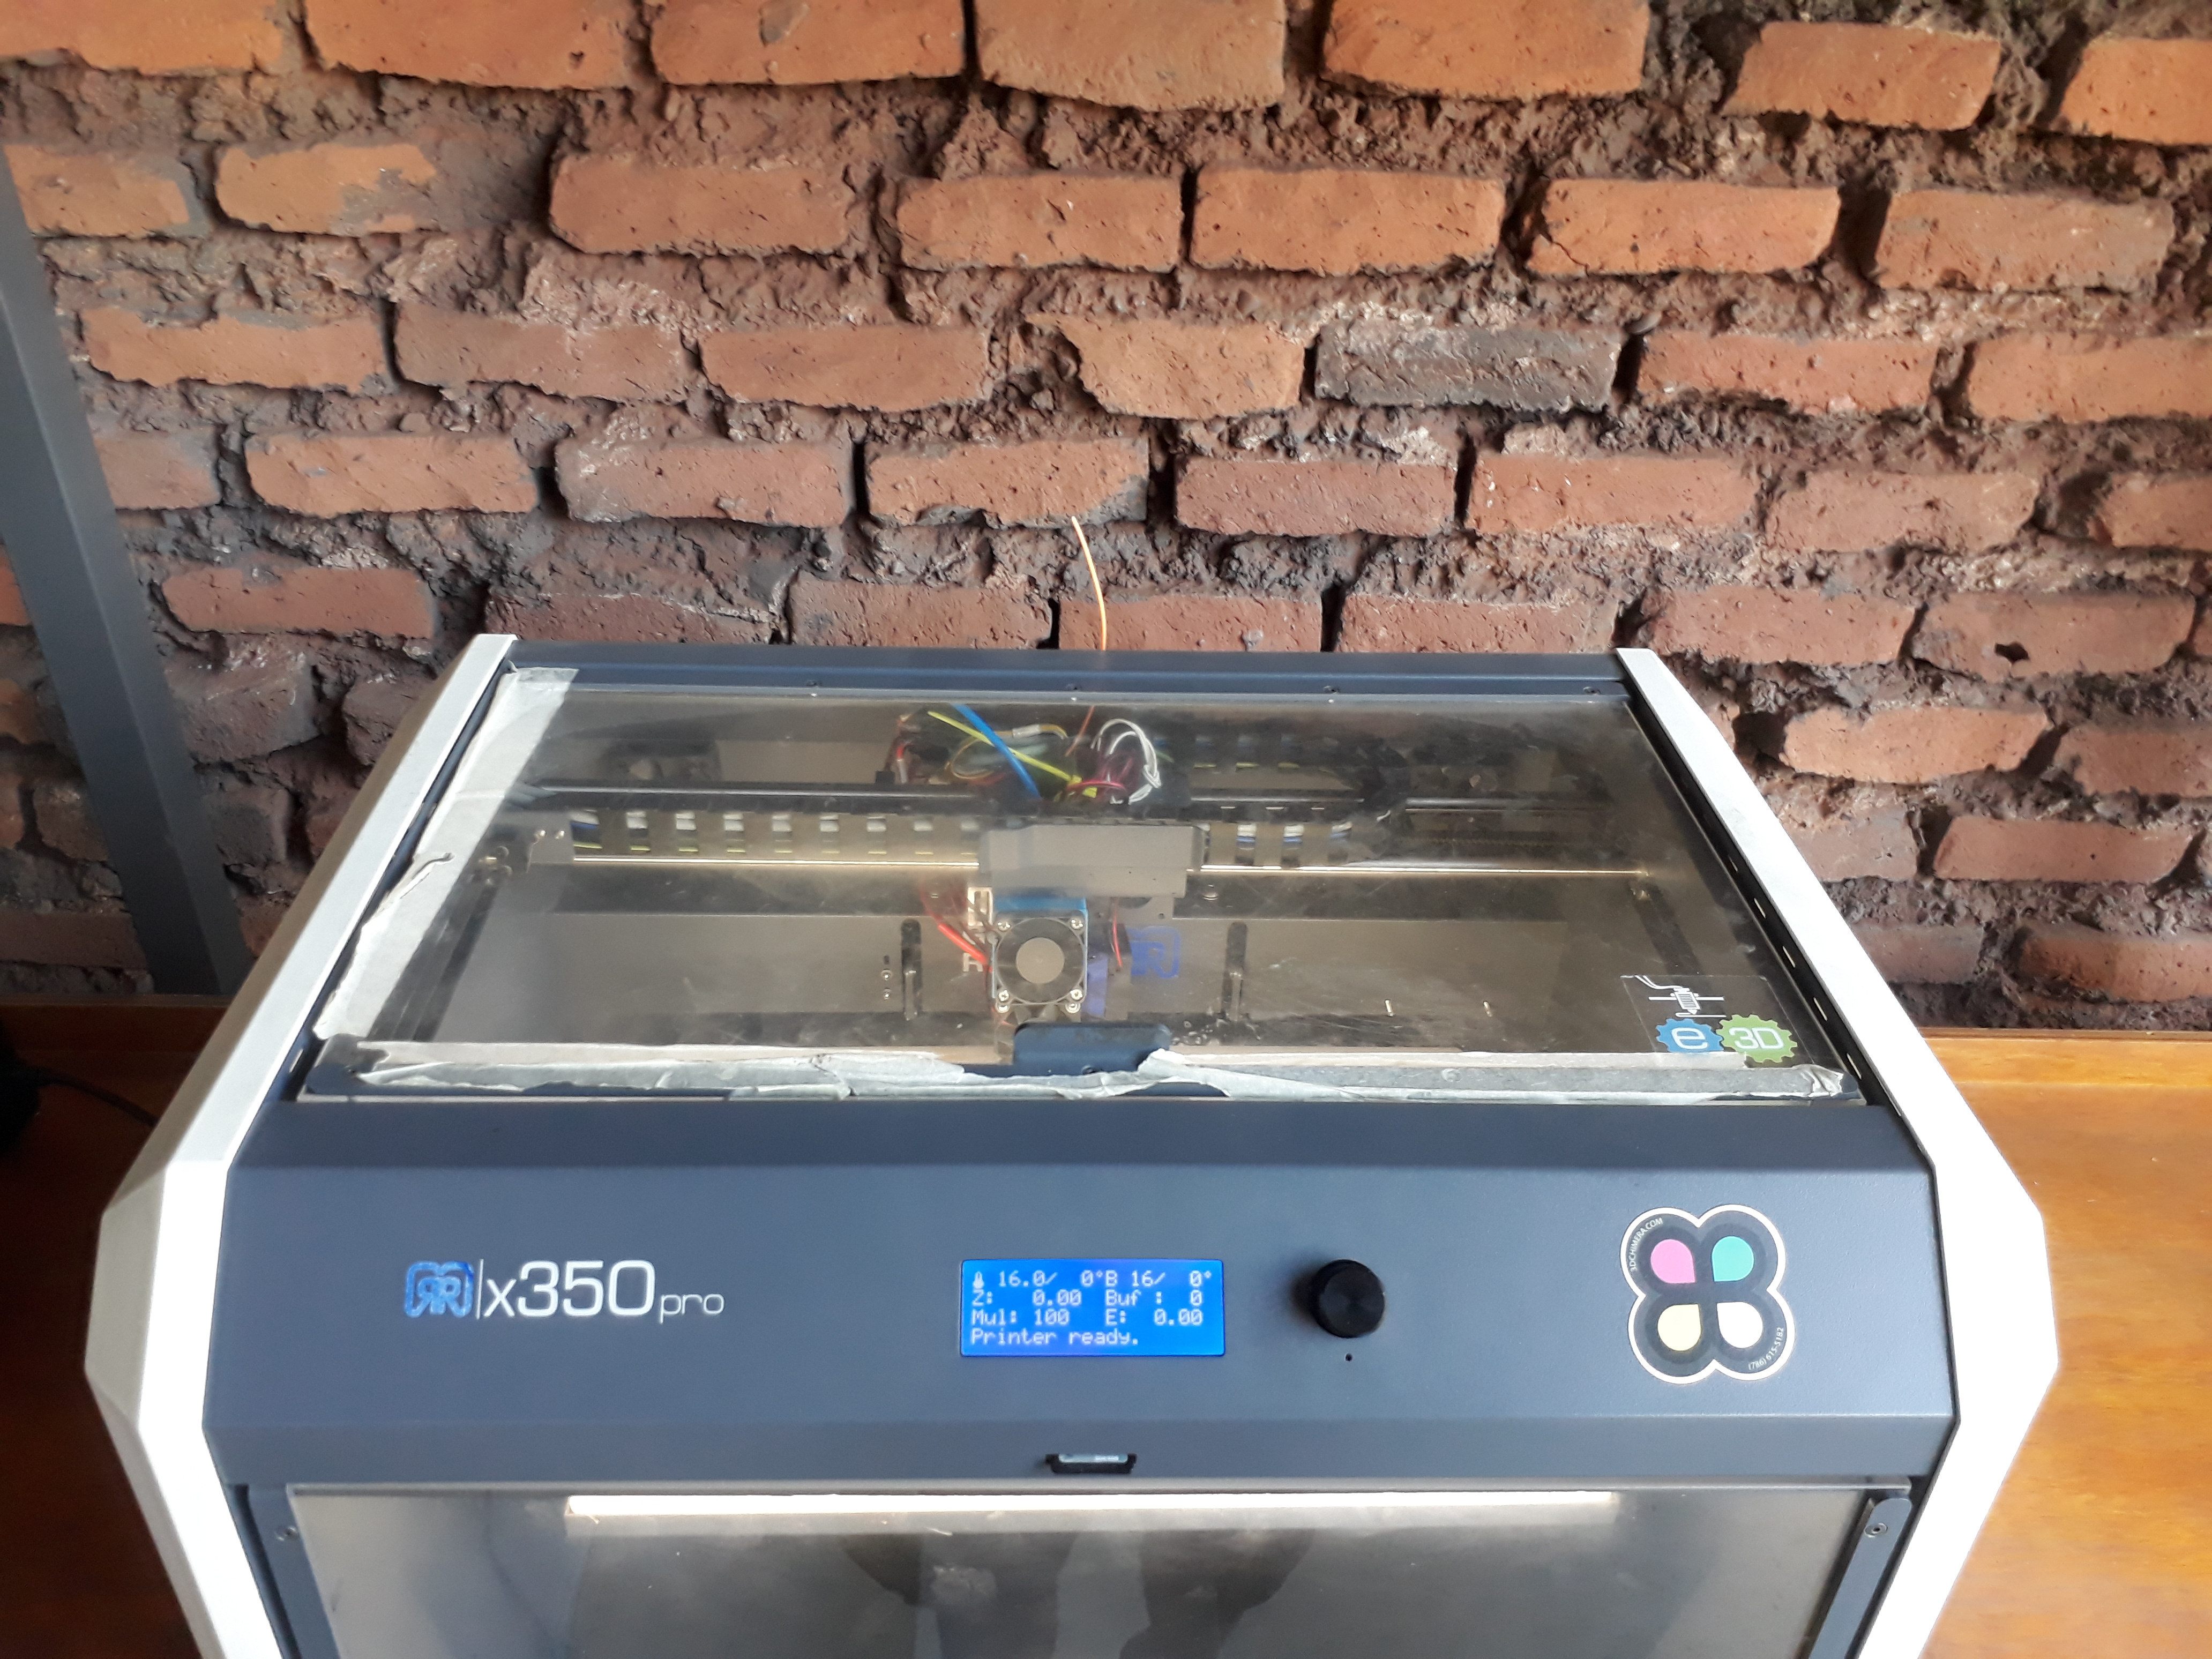
\includegraphics[scale=0.04]{images/x350sup.jpg}\\
\includegraphics[scale=0.04]{images/x350tras.jpg} & \includegraphics[scale=0.04]{images/x350ext.jpg}\\

\end{tabular}
\caption{Impresora X350 desde izquierda a derecha, arriba a abajo: (a) frente; (b) inferior; (c) lateral; (d) superior; (e) trasera; (f) primer plano extrusor.}
\end{table}

Los componentes principales del equipo son:

\begin{itemize}
\item Paneles de chapa metálica: cubierta lateral plegada, que sirve como estructura y bancada de la máquina. Contempla el volumen completo de la impresora, y sirve como barrera térmica para el volumen de fabricación. 
\item Paneles de metacrilato: cubierta superior y barrera frontal de la máquina. Sirve como barrera térmica y está unida a la estructura de chapa metálica por medio de bisagras.
\item Varillas lisas: varillas de acero rectificadas de diámetro 8 mm, cuya función es servir de guía para los ejes del plano x-y. Las varillas del eje-x están unidas a dos carros laterales; las varillas del eje-y están unidas a la estructura de panel de chapa metálica, y soportan los carros del eje-x.
\item Rodamientos lineales: elementos de rodadura para el movimiento en el plano x-y. Están unidas, tanto a los carros del eje-y como al cabezal de impresión en el eje-x.
\item Husillos: barra roscada de diámetro 8 mm y paso 2 mm que sirve como elemento de transmisión de movimiento desde los motores paso a paso a la cama caliente en el eje-z. 
\item Motores Paso a Paso: dispositivo electromecánico que transforma los pulsos eléctricos a movimiento angular. Los motores paso a paso que componen la impresora son del tipo NEMA 17, con una corriente máxima de 1.5 A. Existe uno para generar el movimiento de cada eje.
\item Finales de carrera: dispositivo electrónico que funciona como interruptor del movimientos de los ejes, y limita el recorrido de los ejes x-y-z. Además, la interrupción del movimiento de todos los ejes coincide con el origen de la máquina.
\item Correas GT2: elemento de transmisión de movimiento desde los motores paso a paso a los ejes x-y. la transformación de movimiento angular a lineal se realiza en las poleas dentadas unidas al motor.
\item Cama caliente: superficie de impresión de la impresora 3D compuesta por una resistencia que abarca toda el área. 
\item Termistor: componente electrónico resistivo de 100K, que funciona como sensor de temperatura de extrusor y cama caliente.
\item Extrusor E3D: componente mecánico de empuje de filamento. Está compuesto por piezas que ejercen presión al filamento contra la rueda del motor de extrusión.
\item Difusor: Componente metálico cilíndrico construido con un número específico de aletas, que sirve como disipador térmico del conjunto extrusor.
\item Ventilador de difusor: pequeña turbomáquina que produce un flujo de aire constante contra el difusor, para enfriar de forma eficiente el conjunto extrusor.
\item Ventilador de capa: pequeña turbomáquina que produce un flujo de aire contra la capa en construcción, con el fin de solidificar el plástico apenas es extruido por la boquilla.
\item Garganta: Conducto metálico con hilos en su exterior. Está unido tanto al difusor como al bloque calentador y sirve como conducto para el paso del filamento hasta la zona de calentamiento.
\item Calentador: resistencia de material cerámico de alta potencia, que sirve como elemento calentador para fundir el filamento.
\item Bloque calentador: Bloque metálico que sirve como elemento térmico y de unión entre garganta y boquilla.
\item Boquilla: elemento fabricado en latón o acero con un diámetro de salida menor al de entrada. Es la pieza final del conjunto extrusor y entrega un flujo constante de plástico para la fabricación de la pieza.
\item Placa electrónica: Placa de circuito impreso compuesta por un microcontrolador re-programable y pines de entrada y salida. Este elemento controla la impresora en su conjunto y establece la comunicación entre el microcontrolador, los sensores y actuadores.
\item Interfaz LCD: dispositivo electrónico que muestra información relevante de la impresora en forma gráfica y sirve como elemento de interacción entre el operador y la máquina. Cuenta con una conexión para tarjetas SD, una pantalla LCD y un potenciómetro para controlar la impresora 3D. 
\item Fuente de alimentación: fuente conmutada que trasforma la energía eléctrica de corriente continua a alterna. Alimenta la placa electrónica, los dispositivos electromecánicos y resistivos de la máquina. 
\end{itemize}

La tabla de componentes para la impresora X350 resulta de la siguiente forma:

\begin{table}[H]\centering


\begin{tabular}{|p{1cm}|p{8cm}|p{2cm}|}
\hline
\textbf{ITEM} &\textbf{COMPONENTE} &\textbf{CANTIDAD} \\ \hline
1 &PLACA CONTROLADORA GREPRAP &1 \\ \hline
2 &PANTALLA LCD CON LECTOR PER. SD &1 \\ \hline
3 &DRIVERS A4988 &4 \\ \hline
4 &DISIPADOR DE CALOR PARA DRIVER &4 \\ \hline
5 &FUENTE DE PODER S-360-24 &1 \\ \hline
6 &FUSIBLE 15A 250V 32mm &1 \\ \hline
7 &CABLE 2,5MM NEGRO &1 \\ \hline
8 &CABLE 2,5MM ROJO &1 \\ \hline
9 &CABLE 1MM NEGRO &3 \\ \hline
10 &CABLE 1MM ROJO &3 \\ \hline
11 &CABLES CONECTOR NEMA 17 &8 \\ \hline
12 &CABLES CONECTOR 2PIN 1MM &4 \\ \hline
13 &CABLES CONECTOR 3 PIN 1MM &3 \\ \hline
14 &TIRA LED 24V &1 \\ \hline
15 &FINAL DE CARRERA MECÁNICO &3 \\ \hline
16 &TERMISTOR 100K &2 \\ \hline
17 &HEATBLOCK DYZ &1 \\ \hline
18 &CALENTADOR CAMA 24V &1 \\ \hline
19 &BOQUILLA DYZ &1 \\ \hline
20 &ALUCORE &1 \\ \hline
21 &VENTILADOR 24V 12,5X12,5MM &1 \\ \hline
22 &VENTILADOR 24V 50X50MM &2 \\ \hline
23 &NEMA 17 &3 \\ \hline
24 &EXTRUSOR DYZ &1 \\ \hline
25 &CORREA GT2 &3 \\ \hline
26 &POLEA GT2 &4 \\ \hline
27 &BARRAS LISAS 8MM &6 \\ \hline
28 &BARRAS ROSCADAS 8MM PASO 2MM &1 \\
\hline
29 &RODAMIENTOS LINEALES 8MM &8 \\
\hline
30 &RODAMIENTOS DE BOLA 8MM &2 \\
\hline
31 &SOPORTES ALUMINIO DE BARRAS &4 \\
\hline
32 &CUBIERTA CHAPA METÁLICA &1 \\
\hline
33 &CUBIERTA POLICARBONATO &2 \\
\hline
\end{tabular}
\caption{Tabla de componentes para impresora X350.}
\end{table}

A continuación, se resumen las recomendaciones de mantenimiento y los problemas frecuentes que el fabricante entrega en su guía para el usuario \citep{germanreprap2019}:

\begin{table}[H]
  \centering
 
    \begin{tabular}{|p{9.215em}|p{19.645em}|}
	\hline    
    Problema & \multicolumn{1}{l}{Solución} \\
	\hline    
    El equipo no enciende & Revise la fuente de alimentación \\
	\hline    
    El extrusor no calienta & Revise si la conexión del cable del calentador está bien conectada \\
	\hline    
    la cama no caliente & Revise si la conexión del cable de la cama está bien conectada \\
	\hline    
    La impresora se detiene en medio del proceso & Revise los siguientes ítem: Fuente de poder, tarjeta SD, Gcode inválido \\
	\hline    
    No hay material saliendo de la boquilla, o el flujo es inconsistente & Rectifique la presión de contacto en el extrusor, limpie la boquilla, revise la alimentación de filamento \\
	\hline    
    el objeto en impresión se despega de la cama & Limpie la superficie de construcción. Si es necesario, lubrique la cama con acetona. Verifique la distancia entre la boquilla y la superficie.  \\
	\hline    
    \end{tabular}%
     \caption{Tabla de problemas frecuentes entregados por el fabricante.}
  \label{tab:addlabel}%
\end{table}%


\subsection{Contexto Operacional}

El activo en cuestión realiza sus operaciones en el Taller de Impresión 3Dlux, ubicado en la calle Puma 1180, comuna de Recoleta. Durante los dos años previos a 2020, la máquina operaba junto a otras ocho máquinas impresoras 3D FDM de tipología cartesiana y diversos volúmenes de impresión. Debido al contexto de emergencia sanitaria, se determinó que existirían dos lugares para la producción, reduciendo la cantidad de máquinas en el taller a cuatro. La capacidad de producción de las máquinas se encuentra entre 50 y 80 gramos por hora, dependiendo del material utilizado y otras variables asociadas al proceso de impresión. El recinto es de 55,44 metros cuadrados (6,6x8,8m),el piso  es de carpeta de hormigón y el encielado con aislante térmico de fibra sintética. Cuenta con aislación térmica del exterior a través de muros de albañilería y termopaneles. Asimismo, presenta control de temperatura ambiente a través de una bomba de calor situada a un costado de la entrada al taller. Las máquinas de impresión 3D están situadas en una repisa con base metálica y cubierta de madera contrachapada. La alimentación eléctrica disponible consta de salidas a 220V AC.

\begin{figure}[H]
\centering
\includegraphics[scale=0.4]{images/layout.png}
\caption{Layout y simbología del taller de impresión 3D.}
\end{figure}

\subsection{Delimitación de funciones}

\subsubsection{Diagrama de Interrelaciones Funcionales}

Según \cite{unit2009}, un Diagrama de Interrelaciones Funcionales permite identificar las conexiones lógicas y secuenciales en un producto. En este caso, el diagrama se utiliza para expresar de forma gráfica el funcionamiento de una impresora 3D comprendida como un sistema. Así, se permite representar gráficamente el flujo de variables entre los diversos procesos de un sistema, así también sus entradas y salidas. En el diagrama mostrado a continuación, se representan las interacciones internas y externas en el sistema comprendido por la máquina, y los subsistemas de alimentación, control, construcción, movimiento y extrusión. Asimismo, se observa que si una de las interacciones se ve interrumpida, quiere decir que existe algún tipo de falla en la impresora, y su efecto puede propagarse en la medida que afecte a alguno de los componentes funcionales.

\begin{figure}[H]
\centering
\includegraphics[scale=0.4]{images/diagramafuncional.png}
\caption{Diagrama funcional de bloques para la máquina de impresión 3D.}
\label{diagramafuncional}
\end{figure}

\subsection{Determinación de fallas}

\subsubsection{Árbol de Fallas} 
 
Según \cite{pique1998}, el método de árbol de fallos o FTA por sus siglas en inglés \textit{Fault Tree Analysis} se trata de un método deductivo de análisis que parte de la previa selección de un suceso no deseado o evento que se pretende evitar. Seguidamente, de manera sistemática y lógica se presentan las combinaciones de las situaciones que pueden dar a lugar a la producción del evento a evitar. Se deben conformar niveles sucesivos de tal manera que cada suceso esté generado a partir de sucesos del nivel inferior siendo el nexo de unión entre los niveles la existencia de operadores o puertas lógicas \citep{pique1998}. En la siguiente tabla se muestran los símbolos que se utilizan en el árbol de falla.
 
\begin{table}[H]
\centering
\begin{tabular}{|l|p{7cm}|}
\hline
Símbolo & Significado \\
\hline
\includegraphics[scale=1]{images/arbol/basico.png} & Suceso básico. No requiere de posterior desarrollo al considerarse un suceso de fallo básico. \\ 
\hline
\includegraphics[scale=1]{images/arbol/nodesarrollado.png} & Suceso no desarrollado. No puede ser considerado como básico, pero sus causas no se desarrollan, sea por falta de información o por su poco interés.\\
\hline
\includegraphics[scale=1]{images/arbol/intermedio.png} & Resultante de la combinación de sucesos más elementales por medio de puertas lógicas. Asimismo, se representa en un rectángulo el proceso no deseado del que parte todo el árbol. \\
\hline
\includegraphics[scale=1]{images/arbol/puertay.png} & El suceso de salida ocurrirá si ocurren todos los sucesos de entrada.\\
\hline
\includegraphics[scale=1]{images/arbol/puertao.png} & El suceso de salida ocurrirá si ocurren uno o más de los suceso de entrada\\
\hline
\includegraphics[scale=1]{images/arbol/transferencia.png} & Indica que el árbol continúa en otro lugar. \\
\hline
\end{tabular}
\caption{Símbolos y significados del árbol de fallas \citep{pique1998}}
\end{table}

Según \cite{pique1998}, los pasos para la resolución de árboles de fallo son los siguientes:

\begin{enumerate}
\item Identificar todas las puertas lógicas y sucesos básicos
\item Resolución de todas las puertas en sus sucesos básicos
\item Eliminación de los sucesos repetidos en los conjuntos de fallos.
\item Eliminación de los conjuntos de fallo que contengan a su vez conjuntos de fallo más pequeños.
\end{enumerate}

\begin{figure}[H]
\centering
\includegraphics[scale=0.4]{images/arbol/arbol1.png}
\caption{Árbol de fallas de impresora 3D.}
\end{figure}

\begin{figure}[H]
\centering
\includegraphics[scale=0.4]{images/arbol/arbol2.png}
\caption{Continuación del árbol de fallas de impresora 3D.}
\end{figure}

\begin{figure}[H]
\centering
\includegraphics[scale=0.4]{images/arbol/arbol3.png}
\caption{Continuación del árbol de fallas de impresora 3D.}
\end{figure}

\begin{figure}[H]
\centering
\includegraphics[scale=0.4]{images/arbol/arbol4.png}
\caption{Continuación del árbol de fallas de impresora 3D.}
\end{figure}


\begin{figure}[H]
\centering
\includegraphics[scale=0.4]{images/arbol/arbol5.png}
\caption{Árbol de fallas de impresora 3D.}
\end{figure}

\subsection{Análisis de Modos y Efectos de Falla}

\subsubsection{Estructura del Análisis}

Según la norma SAE JA-1012, un análisis de modos y efectos de fallas puede ayudar a documentar las funciones de un activo, su falla funcional, modos de falla, y los efectos que ésta puede producir. Según \cite{saeja1012}, La descripción debe ser suficientemente detallada de modo que posibilite la selección de una política de manejo de fallas adecuada, pero no tan detallada que tome demasiado tiempo realizar el proceso de análisis. Asimismo, los verbos utilizados para describir los modos de falla se deben seleccionar cuidadosamente, ya que tienen una gran influencia en el proceso de selección de las políticas de manejo de fallas. La estructura propuesta para el análisis se muestra a continuación:


\begin{table}[H]
  \centering
 
    \scalebox{0.6}{\begin{tabular}{|p{15em}|p{8em}|p{9em}|p{9em}|p{8em}|}
    \hline
    \multirow{4}[4]{*}{\textbf{HOJA DE INFORMACIÓN RCM}} & \multicolumn{2}{l|}{\multirow{2}[2]{*}{\textbf{ACTIVO}}} & \multicolumn{2}{l|}{\multirow{2}[2]{*}{\textbf{ACTIVO N°}}} \\
    \multicolumn{1}{|c|}{} & \multicolumn{2}{l|}{} & \multicolumn{2}{l|}{} \\
   \multicolumn{1}{|c|}{} & \multicolumn{2}{l|}{\multirow{2}[2]{*}{\textbf{SUBSISTEMA}}} & \multicolumn{2}{l|}{\multirow{2}[2]{*}{\textbf{SUBSISTEMA N°}}} \\
    \multicolumn{1}{|c|}{} & \multicolumn{2}{l|}{} & \multicolumn{2}{l|}{} \\
    \hline
    \textbf{COMPONENTE} & \textbf{FUNCIÓN} & \textbf{FALLA FUNCIONAL} & \textbf{MODO DE FALLA} & \textbf{EFECTOS DE LAS FALLAS} \\
    \hline
    \end{tabular}}
    
    \caption{Estructura propuesta para hoja de Información RCM.}
  \label{tab:addlabel}%
\end{table}%

\subsubsection{Estructura Diagrama de decisión}

Si bien la norma SAE JA1012 entrega diagramas tipo para la elaboración del diagrama de decisión RCM, deja de manifiesto que existen diferencias entre los distintos tipos de diagramas utilizados en el mundo, llegando a siquiera cumplir con la normativa SAE JA1011 en algunos casos. Es por esto que, para la realización de esta herramienta, se realiza una búsqueda con el fin de encontrar un algoritmo de de decisión afín al tipo de mantenimiento que se busca hacer en este caso. En todo caso, según \cite{saeja1012}, las fases de aplicación de este diagrama se conforma típicamente por tres fases:

\begin{enumerate}
\item Trabajando desde el principio, utilice el diagrama de decisión para determinar las categorías de consecuencias que aplica al modo de falla en consideración.
\item Luego trabajando con la columna de consecuencias relevantes, utilice el criterio de factibilidad técnica de las posibles políticas de manejo de fallas en cada categoría.
\item Seleccione una política de manejo de fallas desde la primera categoría que satisfaga el criterio de factibilidad técnica y que tratará con las consecuencias del modo de falla en consideración.

\end{enumerate}

El diagrama de decisión utilizado en este caso, se muestra a continuación:

\begin{figure}[H]
\centering
\includegraphics[scale=0.45, angle=90]{images/decisionrcm.png}
\caption{Diagrama de decisión para impresora 3D.}
\end{figure}


Por otra parte, la estructura para la hoja de decisión RCM es la siguiente:


\begin{table}[H]
  \centering
  
    \scalebox{0.4}{\begin{tabular}{|l|l|l|l|l|l|l|l|l|l|l|l|l|c|c|c|}
    \hline
    \multicolumn{7}{|c|}{\multirow{3}[4]{*}{\textbf{HOJA DE DECISIÓN RCM}}} & \multicolumn{6}{l|}{\textbf{SISTEMA/ACTIVO}}  & \multicolumn{3}{l|}{\textbf{ACTIVO N°}} \\
\cline{8-16}    \multicolumn{7}{|c|}{}                                & \multicolumn{6}{l|}{\multirow{2}[2]{*}{\textbf{SUBSISTEMA}}} & \multicolumn{3}{l|}{\multirow{2}[2]{*}{\textbf{SUBSISTEMA N°}}} \\
    \multicolumn{7}{|c|}{}                                & \multicolumn{6}{l|}{}                         & \multicolumn{3}{l|}{} \\
    \hline
    \multicolumn{3}{|c|}{\multirow{3}[6]{*}{Referencia de Información}} & \multicolumn{4}{c|}{\multirow{3}[6]{*}{Evaluación de consecuencias}} & H1    & H2    & H3    & \multicolumn{3}{c|}{\multirow{3}[6]{*}{Tareas a falta de}} & \multicolumn{1}{c|}{\multirow{4}[8]{*}{Tareas Propuestas}} & \multicolumn{1}{c|}{\multirow{4}[8]{*}{Frecuencia Inicial}} & \multicolumn{1}{c|}{\multirow{4}[8]{*}{A  realizar por}} \\
\cline{8-10}    \multicolumn{3}{|c|}{} & \multicolumn{4}{c|}{}         & S1    & S2    & S3    & \multicolumn{3}{c|}{} &       &       &  \\
\cline{8-10}    \multicolumn{3}{|c|}{} & \multicolumn{4}{c|}{}         & O1    & O2    & O3    & \multicolumn{3}{c|}{} &       &       &  \\
\cline{1-13}    F     & FF    & MF    & H     & S     & E     & O     & N1    & N2    & N3    & H4    & H5    & S4    &       &       &   \\
    \hline
    \end{tabular}}%
    \caption{Estructura propuesta para hoja de Información RCM.}
  \label{tab:addlabel}%
\end{table}%

\subsubsection{Resultados}

A continuación, se muestran las hojas de información RCM obtenidos para los subsistemas comprendidos en la figura \ref{diagramafuncional}.

\begin{figure}[H]
\centering
\includegraphics[scale=0.8]{images/amef1.png}
\caption{Hoja de información RCM para subsistema de extrusión de impresora X350.}
\end{figure}
\begin{figure}[H]
\centering
\includegraphics[scale=0.8]{images/amef2.png}
\caption{Continuación de hoja de información RCM para subsistema de extrusión de impresora X350.}
\end{figure}

\begin{figure}[H]
\centering
\includegraphics[scale=0.8]{images/amef3.png}
\caption{Continuación de hoja de información RCM para subsistema de extrusión de impresora X350.}
\end{figure}
\begin{figure}[H]
\centering
\includegraphics[scale=0.7]{images/decision1.png}
\caption{Hoja de decisión RCM para subsistema de extrusión de impresora X350}
\end{figure}

\begin{figure}[H]
\centering
\includegraphics[scale=0.7]{images/decision2.png}
\caption{Continuación de hoja de decisión RCM para subsistema de extrusión de impresora X350}
\end{figure}
\begin{figure}[H]
\centering
\includegraphics[scale=0.7]{images/decision3.png}
\caption{Continuación de hoja de decisión RCM para subsistema de extrusión de impresora X350}
\end{figure}

\begin{figure}[H]
\centering
\includegraphics[scale=0.8]{images/amef21.png}
\caption{Hoja de información RCM para subsistema de movimiento de impresora X350.}
\end{figure}
\begin{figure}[H]
\centering
\includegraphics[scale=0.8]{images/amef22.png}
\caption{Continuación de hoja de información RCM para subsistema de movimiento de impresora X350.}
\end{figure}

\begin{figure}[H]
\centering
\includegraphics[scale=0.8]{images/amef23.png}
\caption{Continuación de hoja de información RCM para subsistema de movimiento de impresora X350.}
\end{figure}
\begin{figure}[H]
\centering
\includegraphics[scale=0.7]{images/decision21.png}
\caption{Hoja de decisión RCM para subsistema de movimiento de impresora X350}
\end{figure}

\begin{figure}[H]
\centering
\includegraphics[scale=0.7]{images/decision22.png}
\caption{Continuación de hoja de decisión RCM para subsistema de movimiento de impresora X350}
\end{figure}

\begin{figure}[H]
\centering
\includegraphics[scale=0.7]{images/amef31.png}
\caption{Hoja de información RCM para subsistema de control de impresora X350}
\end{figure}

\begin{figure}[H]
\centering
\includegraphics[scale=0.7]{images/decision31.png}
\caption{Hoja de decisión RCM para subsistema de control de impresora X350}
\end{figure}

\begin{figure}[H]
\centering
\includegraphics[scale=0.65]{images/amef41.png}
\caption{Hoja de información RCM para subsistema de alimentación de impresora X350}
\end{figure}

\begin{figure}[H]
\centering
\includegraphics[scale=0.7]{images/decision41.png}
\caption{Hoja de decisión RCM para subsistema de alimentación de impresora X350}
\end{figure}

\begin{figure}[H]
\centering
\includegraphics[scale=0.7]{images/amef51.png}
\caption{Hoja de información RCM para subsistema de construcción de impresora X350}
\end{figure}

\begin{figure}[H]
\centering
\includegraphics[scale=0.7]{images/amef52.png}
\caption{Continuación de hoja de información RCM para subsistema de construcción de impresora X350}
\end{figure}


\begin{figure}[H]
\centering
\includegraphics[scale=0.7]{images/decision41.png}
\caption{Hoja de decisión RCM para subsistema de construcción de impresora X350}
\end{figure}



\section{Aplicación de metodología Design Thinking para el desarrollo de Aplicación Web}

En esta sección de detallará la implementación, marco de trabajo y aplicación de la metodología de Design thinking que busca obtener mejoras en los procesos de la gestión de la producción y el mantenimiento en impresoras 3D FDM a través del desarrollo y pruebas de una aplicación web. En primer lugar, se define la situación actual de la empresa, y posteriormente se detallan los pasos para la implementación del marco de trabajo propuesto para cada fase de la metodología.

\subsection{Situación actual}

Actualmente, la empresa posee un proceso definido para la recepción, producción y entrega de piezas y productos que involucra tanto al operador, la máquina de impresión y un computador donde se realiza el tratamiento de los archivos. Este proceso a grandes rasgos, consiste en la recepción y evaluación de lo solicitado por el cliente, definir si solo contempla servicios de impresión 3D u otros adicionales (diseño 3D para otros procesos, escáner 3D, post-procesos de piezas, entre otros), ejecución del o los servicios, y confirmación de despacho al cliente.  

\begin{figure}[H]
\centering
\includegraphics[scale=0.4]{images/procesosdiag.png}
\caption{Diagrama de flujos para el proceso de recepción, producción y entrega de piezas y productos.}
\label{procesosdiag}
\end{figure}


Específicamente, el interés de aplicación de la metodología es la mejora del proceso de la producción y el mantenimiento, por tanto se delimita el marco de trabajo a estos pasos específicos del flujo, tal como se muestra en la figura \ref{procesosdiag}. Así, se puede representar según el siguiente orden.

\begin{itemize}
\item Exportación de la pieza a lenguaje estándar de triángulos (.stl).
\item Configuración de variables de impresión en software CAM.
\item Exportación de la pieza en formato .gcode.
\item Carga de archivo en la máquina.
\item Precalentamiento de la máquina.
\item Fabricación de la pieza.
\item Extracción de la pieza y post-proceso en caso de ser necesario.
\end{itemize}

El diagrama de flujo que representa el proceso, decisiones y resultados, se muestra en la figura \ref{proceso}

\begin{figure}[H]
\centering
\includegraphics[scale=0.4]{images/proceso.png}
\caption{Diagrama de flujo del proceso de impresión 3D.}
\label{proceso}
\end{figure}

Se observa que durante el proceso existen, a lo menos, tres escenarios o lugares para la producción de una pieza. En primer lugar, se nota que todo el tratamiento del archivo se realiza en un solo computador bajo la utilización de dos softwares simultáneos, en este caso, el programa de diseño CAD y el laminador CAM. El laminador, además de convertir el archivo a un formato legible para la máquina, entrega ciertos parámetros que sirven como insumo para estimar los costos de producción, como el peso del filamento utilizado en la fabricación y el tiempo que eventualmente tardaría en terminar la operación. Luego, el archivo en formato Gcode es almacenado en una tarjeta SD y extraído del computador para ser llevado físicamente hasta la máquina de impresión 3D; en este lugar, el operador carga la tarjeta y realiza las tareas previas para la impresión del archivo, ya sea la inspección visual, limpieza del conjunto extrusor y las superficie de construcción, y el precalentamiento de la cama según el material realizado. Finalmente, al término de la operación la interfaz de la impresora muestra el tiempo efectivo de construcción, y comienza a enfriar los elementos térmicos con el fin de facilitar la extracción de la pieza; en este momento, el operador saca las piezas, verifica que cumplan con los requerimientos especificados y desecha los objetos que, producto del proceso, resultaron fallidos o fuera de especificación. 

\subsection{Planificación del marco de trabajo}

Para definir el rumbo de planificación del proyecto, se estima conveniente trabajar en seis fases inspiradas en el design tinking: empatizar, definir, investigar, idear, prototipar y testear. De esta forma, el marco de trabajo se resume de la siguiente forma:

\begin{table}[H]
\centering
\begin{tabular}{|p{3.5cm}|p{3.5cm}|p{3.5cm}|}
\hline
Etapa & Hito & Características \\
\hline
Empatizar & detectar problemática & Mapa skateholders,entrevista personal, journey map \\
\hline
Definir & Definición de necesidades del usuario & 5W, obtención de \textit{insight}\\
\hline
Investigar & Conocimiento de referentes y herramientas de desarrollo & Investigación de referentes y herramientas \\
\hline
Idear & Obtener propuestas de desarrollo & lluvia de ideas \\
\hline
Prototipar & Estructurar la información, interfaz de usuario & prototipos estéticos y funcionales \\
\hline
Testear & prueba en entorno de producción & aplicación funcional \\
\hline

\end{tabular}
\caption{Tabla resumen del marco de trabajo y sus características.}
\end{table}

\subsection{Empatizar}

La fase de inicio consiste en investigar cómo y por qué los usuarios, en este caso todos las personas involucradas en el proceso de impresión 3D, realizan las acciones que ellos encuentran determinantes en el proceso de impresión. Según la metodología, estos son definidos como \textit{stakeholders}. Este paso es indispensable, pues revela las personalidades, necesidades y patrones de trabajo de los stakeholders, y solo así se puede comenzar a esbozar el diseño de un concepto de producto en el cual se orientará la aplicación. Esto se realiza a través de un \textit{mapa de stakeholders}. Así, se reconoce que el principal sujeto de análisis es el operario de la impresora 3D. En la misma línea, otros participantes que tienen conexión con el proyecto son el diseñador y quien se encarga de la gestión de la empresa. Se consideran como contribuyentes o beneficiarios indirectos a los clientes de la empresa y quienes prestan servicios o insumos; también se encuentran indirectamente los competidores con capacidad similar de producción.

\begin{figure}[H]
\centering
\includegraphics[scale=0.4]{images/stakeholders.png}
\caption{Mapa de Stakeholders del proyecto.}
\end{figure}

Considerando el resultado obtenido, se solicitó realizar una entrevista al operario de las máquinas con el fin de obtener información respecto a su visión de usuario respecto a entender su visión como usuario de impresoras 3D, su percepción de la actual acción y gestión del mantenimiento, la forma en que realiza el mantenimiento a las máquinas, y conocer sus canales de proveedores. El resultado de la entrevista se sistematiza en la siguiente tabla:


\begin{table}[H]
\begin{tabular}{|p{5cm}|p{8cm}|}
\hline
Presentación, ocupación y cargo & Su nombre es Javier Oliva, es cofundador de 3Dlux y diseñador de profesión.  \\
\hline
Tareas relacionadas con impresión 3D & La tareas que realiza  se relacionan a la administración, marketing y fabricación de piezas 3D, además de post proceso de piezas en caso de ser necesario.\\
\hline 
Importancia de sistemas de gestión de Mantenimiento & Bastante importante, pues estandariza proceso y existe mayor control. Piensa que es positivo adelantarse a las fallas y mantener las máquinas en buen estado dada su experiencia en pedidos grandes o con tiempo limitado \\
\hline
Realización de mantenimientos & Si ha realizado mantenimientos \\ 
\hline
Problemas relacionados con el mantenimiento & Ha tenido problemas en el desconocimiento de algunas piezas, o manejar piezas electrónicas.\\
\hline
Herramientas de gestión & No ocupa ninguna herramienta para gestionar el mantenimiento. \\
\hline
Mantenimiento preventivo o correctivo & En mayor proporción espera a que un componente falle. El mantenimiento preventivo no está calendarizado, sino que se realiza antes de trabajos largos.\\
\hline
Clasificación de fallas & No especifica las fallas que ocurren. Busca identificar el problema según algún subsistema de la impresora, mecánico o electrónico, por ejemplo.\\
\hline
Utilidad de registros de mantenimiento & Encuentra mucha utilidad a los registros, pues sería más sencillo facilitar la tarea a quienes puedan conformar el grupo.\\
\hline
Información relevante para el negocio & Cree relevante el detectar los tipos de falla y el procedimiento más óptimo.\\
\hline
Comunicación con proveedores & Si tiene comunicación con proveedores. No existe solo uno, sino que dependen de la oportunidad de compra.\\
\hline
Uso de Octoprint & Lo ha utilizado, pero cree que la configuración puede ser difícil en ocasiones. Sin embargo, piensa que puede ser una buena alternativa en caso que se pueda relacionar con los registros.\\
\hline
\end{tabular}
\caption{Resumen de respuestas dadas por el operario de mantenimiento en entrevista.}
\end{table}







Una forma de obtener las vivencias del operario en su recorrido durante el proceso de impresión 3D es utilizando el mapa de experiencia o \textit{customer journey map}. Esta herramienta permite obtener información sobre cada etapa del proceso, conociendo los objetivos, actividad, puntos de contacto, sentimientos, emociones, además de obtener conclusiones que puedan surgir como oportunidad a partir de los resultados. En este caso, el mapa de experiencia pretende apoyaren la mejora de las labores que se están realizando actualmente respecto al buen estado de las máquinas en una granja de impresoras 3D con 9 máquinas. Muchas veces, no existe control sobre los pedidos grandes, entregando piezas defectuosas o en cantidades erróneas. Asimismo, debido a fallas de distinto tipo, los pedidos se atrasan en su plazo de entrega. También, las máquinas fallan y no se encuentran disponibles para realizar trabajos. Esta herramienta será usada por quien realiza esta tesis, con el fin de desarrollar herramientas digitales para mejorar y estandarizar el proceso de impresión 3D, y también mantener las máquinas disponibles y en buen estado. Los mapas de experiencia tratan de la experiencia de Javier Oliva, operario de impresoras 3D, quien a su vez está encargado de la gestión de la producción, y fueron realizados en el taller de la empresa. A continuación, se definen las etapas que se evaluarán:

\begin{enumerate}
\item Preparación de archivos.
\begin{enumerate} 
\item Abrir archivo .stl.
\item Guardar archivo Gcode y extraer tarjeta SD.
\end{enumerate}
\item Preparación de la impresora.
\begin{enumerate}
\item Encendido y limpieza general de la impresora.
\item Preparación de la impresora.
\item Insertar SD e imprimir archivo Gcode.
\end{enumerate}
\item Finalización de la impresión.
\begin{enumerate}
\item Control visual de la impresión.
\item Término del proceso.
\item Control visual y registro de piezas.
\end{enumerate}

\begin{figure}[H]
\includegraphics[scale=0.55]{images/jm1.png}
\caption{Primera etapa del mapa de experiencia.}
\end{figure}
\begin{figure}[H]
\includegraphics[scale=0.55]{images/jm2.png}
\caption{Segunda etapa del mapa de experiencia.}
\end{figure}
\begin{figure}[H]
\includegraphics[scale=0.55]{images/jm3.png}
\caption{Tercera etapa del mapa de experiencia.}
\end{figure}

\end{enumerate}

Del análisis realizado a través del mapa de experiencia, se obtienen las siguientes conclusiones en función de sus fases:

\begin{itemize}
\item Preparación de archivos
\begin{itemize}
\item Podría existir una oportunidad de mejora al saber el estado de la máquina a utilizar respecto a los fallos anteriores, y obtener el tiempo de impresión real.
\item Una oportunidad de mejora es establecer un estándar para el nombre de los archivos que se guardarán. Asimismo, explorar posibilidades que puedan suplir el uso de la tarjeta micro SD y que sean confiables.
\end{itemize}
\item Preparación de la impresora
\begin{itemize}
\item Se plantea como mejora el poder configurar el precalentamiento desde el mismo lugar desde donde se configuran los archivos, con el fin de disminuir el tránsito entre la estación de trabajo y la máquina.
\item Una oportunidad de mejora está en poder cargar los archivos desde el mismo espacio de trabajo, con el fin de reducir la inspección de la impresora solo al momento del encendido y construcción de primera capa.
\end{itemize}
\item término del proceso de impresión
\begin{itemize}
\item Se puede obtener una mejora al poder registrar automáticamente las veces en que una impresión está terminada, así como el tiempo que demoró, y la marca temporal en que ocurre el suceso.
\item Existe una oportunidad de mejora al poder realizar un asistente de registro que libere al usuario de tener que abrir planillas para el registro, así como tener un acceso fácil a estos. 
\end{itemize}
\end{itemize}

\subsection{Definir}
Para comprender y definir los requisitos de diseño para la solución propuesta y, al mismo tiempo, transformarlos en objetivos de diseño, es trabaja con la técnica de las \textit{cinco W}. Este se sintetiza desde la entrevista con el usuario, la cual arroja los siguientes resultados:

\begin{table}[H]
\centering
\begin{tabular}{|p{5cm}|p{5cm}|}
\hline
Pregunta & Resultados \\
\hline
¿Quién es el cliente y el público objetivo? &  Operador de granja de impresión 3D que cumple más responsabilidades, como gestión de la producción, reparación y administración de la empresa\\
\hline
¿En qué solución del diseño piensa el cliente? & aplicaciones que puedan ser utilizadas desde computador o dispositivo móvil \\
\hline
¿Cuándo y por cuánto tiempo será necesitado el diseño & No existe un límite inicial, se pretende utilizar durante el tiempo en que las máquinas se encuentren operativas.\\
\hline
¿Dónde será utilizado el diseño? & En el taller de impresión 3D de 3Dlux, a través de una interfaz como un computador o dispositivo móvil \\
\hline
¿Cómo será implementada la solución? & de manera gradual, hasta completar la mayor cantidad de impresoras 3D.\\
\hline
\end{tabular}
\caption{Resultados de la técnica de las cinco W.}
\end{table}



De las técnicas anteriormente utilizadas, y a modo de conseguir los \textit{insight} o los porqués detrás de las necesidades del usuario, se obtiene lo siguiente:

\begin{itemize}
\item El usuario cree importante tener un sistema de gestión y de registros, pues vislumbra mayor control de lo que se está haciendo.
\item Al usuario le preocupa que la información referida al proceso de impresión no suele ser correcta (los tiempos son infravalorados y el tiempo real siempre es mayor al tiempo entregado por el software CAM).
\item Existe preocupación a que no se puedan realizar los registros debido a que existe mucho tránsito entre el espacio de trabajo y el banco de impresoras.
\item Al usuario le resulta frustrante la manipulación excesiva de la tarjeta SD para efectuar la fabricación. 
\item El usuario se siente satisfecho con la limpieza de las impresoras, pues es fácil y rápido, y no suelen haber problemas en torno a esto.
\item Al usuario le preocupa una planificación incorrecta del trabajo, que pueda provocar demoras en la fabricación.
\item Al usuario le resulta tedioso tener múltiples aplicaciones abiertas (planillas, carpetas, programas de uso en el trabajo), y no poder registrar en pocos pasos la producción.
\end{itemize}




\subsection{Investigar}

En esta etapa se busca obtener la mayor información posible respecto a la tecnologías desarrolladas para la gestión de los procesos de mantenimiento, ya sea para pequeñas y medianas empresas, industrias y manufactura aditiva. Para esto, se realiza una investigación del tipo secundaria a partir de información obtenida por fuentes externas, y cualitativa en la medida que pueda informar respecto al consumo de tecnologías de gestión. Para esto, se proponen tres tipos de investigación:

\begin{itemize}

\item Investigación de referentes 
\item Investigación de softwares a utilizar
\item Investigación de las herramientas de desarrollo a utilizar.
\end{itemize}

\subsubsection{Investigación de referentes}

La investigación de referentes estará centrada en softwares o aplicaciones de gestión de la producción y/o mantenimiento disponibles en el mercado mundial. Se elegirán tres empresas que prestan este tipo de servicio, según: (a) vinculación con la impresión 3D; (b) relación con el mantenimiento; (c) relación a la producción. Asimismo, los criterios para el análisis se centran en:
\begin{itemize}
\item Público objetivo
\item Interfaz de monitoreo de condición
\item Interfaz de mantenimiento de activos
\item Interfaz de producción y procesos

\end{itemize}

\paragraph{3Dtrust - https://3dtrust.de/}

\textit{3dtrust} es una empresa de cinco años de antiguedad fundada en Munich, Alemania. Al principio, el equipo formaba parte de una serie de nuevas empresas que querían asegurar la cadena de suministro digital. Según la empresa, a través del cifrado y el software las empresas podían asegurarse de que estaban imprimiendo las piezas correctas. A través del desarrollo de productos y el contacto con el mercado, la empresa ha crecido hasta  crear un software que puede realizar la trazabilidad, la optimización de la productividad y analizar flotas enteras de sistemas de aditivos que producen piezas a tiempo, así como los pasos de posproducción, para decidir qué se debe hacer.

\begin{figure}[H]
\centering
\includegraphics[scale=1]{images/3dtmonitoreo.png}
\caption{Captura de interfaz utilizada por \textit{3Dtrust} para el monitoreo de la condición.}
\label{3dtmonitoreo}
\end{figure}

\begin{figure}[H]
\centering
\includegraphics[scale=1]{images/3dtmonitoreo2.png}
\caption{Captura de interfaz utilizada por \textit{3Dtrust} para el monitoreo de la condición.}
\label{3dtmonitoreo2}
\end{figure}

\begin{figure}[H]
\centering
\includegraphics[scale=1]{images/3dtmonitoreo3.png}
\caption{Captura de interfaz utilizada por \textit{3Dtrust} para el control de la producción.}
\label{3dtmonitoreo3}
\end{figure}

\paragraph{AMFG - https://amfg.ai/service-bureaus-2/}

\textit{AMFG} En el sector de la impresión 3D, la empresa londinense AMFG ofrece un software de automatización de flujo de trabajo de manufactura aditiva para empresas. Su software es una solución de gestión de flujo de trabajo completa e integral. AMFG es la única plataforma de software que ofrece una solución completa de automatización de extremo a extremo para las operaciones

\begin{figure}[H]
\centering
\includegraphics[scale=1]{images/amfg.png}
\caption{Captura de interfaz utilizada por \textit{AMFG} para el control de la producción}
\label{amfg}
\end{figure}

\begin{figure}[H]
\centering
\includegraphics[scale=0.9]{images/amfg2.png}
\label{amfg2}
\caption{Captura de interfaz utilizada por \textit{AMFG} para el control de la producción.}
\end{figure}

\paragraph{FRACCTAL - https://www.fracttal.com/es/}

\textit{FRACCTAL} es una empresa fundada en Chile el año 2014 con el fin de crear un software de mantenimiento y gestión de activos accesibles a medianas y pequeña empresas. Actualmente, su software es utilizado por empresas como Unilever, Aguas Andinas y Petrobras.

\begin{figure}[H]
\centering
\includegraphics[scale=0.9]{images/fracctal.png}
\caption{Captura de interfaz utilizada por \textit{FRACCTAL} para el control de indicadores.}
\label{fracctal}
\end{figure}


\begin{figure}[H]
\centering
\includegraphics[scale=0.9]{images/fracctal2.png}
\caption{Captura de interfaz utilizada por \textit{FRACCTAL} para el control del mantenimiento.}
\label{fracctal2}
\end{figure}

\begin{figure}[H]
\centering
\includegraphics[scale=0.9]{images/fracctal2.png}
\caption{Captura de interfaz utilizada por \textit{FRACCTAL} para la gestión de tareas.}
\label{fracctal3}
\end{figure}

En primer lugar, se nota que el público objetivo de todas las empresas corresponde a pequeñas, medianas y grandes industrias de manufactura. Como se observa en las figuras \ref{3dtmonitoreo} y \ref{3dtmonitoreo2}, en el caso de \textit{3DTrust} el monitoreo de la condición se realiza a través de dos interfaces distintas, una para la la observación de los estados de temperatura de una impresora 3D a lo largo del tiempo, y otra a modo de \textit{dashboard} para el monitoreo de las máquinas conectadas. En la figura \ref{3dtmonitoreo3}, se muestra que la forma de gestionar el control de la producción es a través de las funciones básicas de las bases de datos denominada \textit{CRUD},por el acrónimo en inglés de las funciones leer, actualizar, eliminar o crear. Por otra parte, \textit{AMFG} opta por realizar un calendario de actividades para la gestión de la producción. En la figura \ref{amfg} se muestra una interfaz gráfica para representar el estado y el tiempo de realización de las tareas planificadas. Además, existe la posibilidad de verificar el modelo a imprimir en la misma aplicación, tal como se observa en la figura \ref{amfg2}. En relación a \textit{FRACCTAL}, la principal cualidad es que en su \textit{dashboard} entrega información a modo de indicadores, ya sea gráficos o escalas, del cumplimiento de las tareas propuestas. En la figura \ref{fracctal} se pueden encontrar indicadores de porcentaje de cumplimiento, tareas planificadas versus no planificadas, entre otros. Al igual que con la empresa anterior, la sección relacionada a acciones y control de mantenimiento se realiza a través de funciones \textit{CRUD}, y se muestra a través de una interfaz de base de datos; esta característica se repite respecto al sistema de gestión de tareas, como se observa en la figura \ref{fracctal3}.


\begin{table}[H]
\centering
\begin{tabular}{|p{2.5cm}|p{3.4cm}|p{3.4cm}|p{3.4cm}|}
\hline
Criterio & 3DTrust & AMFG & FRACCTAL \\
\hline
Público Objetivo & Medianas y grandes empresas de la industria de manufactura en impresión 3D& Grandes empresas de la manufactura aditiva & Pequeñas, medianas y grandes empresas de la industria y logística\\
\hline
Relación con impresión 3D & Software diseñado para impresión 3D & Software diseñado para impresión 3D & Se puede implementar en algunos proceso de la impresión 3D \\
\hline
Mantenimiento de activos & Presenta monitoreo de la condición a través del control permanente de algunas variables & Presenta monitoreo de la condición a través del control permanente de algunas variables & Permite la gestión de los registros de mantenimiento a través de operaciones de bases de datos y la obtención de indicadores para el mantenimiento.\\
\hline

Gestión de los procesos & Es posible controlar y gestionar la producción a través de operaciones de bases de datos & Es posible controlar y gestionar la producción a través de la calendarización de la fabricación & Es posible controlar y gestionar la producción a través de operaciones de bases de datos\\
\hline
\end{tabular}
\caption{Tabla resumen del análisis de referentes según los criterios propuestos.}
\end{table}

\subsubsection{Investigación de software a utilizar}

Según \cite{marchante2020}, \textit{OctoPrint} es una aplicación de código abierto y gratuita para el control de impresoras 3D. Permite administrar todas tus impresiones de forma remota y controlar el parque de máquinas con total tranquilidad. Funciona directamente desde su interfaz web, solo hay que conectar la aplicación a la red local. Concretamente, permitirá enviar varios archivos Gcode a diferentes máquinas a través de una única interfaz. La mayoría de los usuarios ahora lo instalan en una Raspberry Pi, usando la imagen OctoPi disponible en línea. OctoPrint también es compatible con cámaras que permitirán el monitoreo en tiempo real de una impresión y verificar de forma remota que todo funciona correctamente.En 2012, Gina Häußge desarrolló una primera aplicación de control, utilizando su propia impresora 3D. Muy rápidamente, la solución sedujo al mercado y fue el fabricante español BQ quien apoyó financieramente el desarrollo. Hoy, OctoPrint es ampliamente utilizado en todo el mundo, es de código abierto y completamente gratuito. Incluso se ha creado un foro para reunir a toda la comunidad de usuarios, resolver problemas técnicos, facilitar la instalación de la aplicación o intercambiar ideas.

\begin{figure}[H]
\centering
\includegraphics[scale=0.5]{images/octoprint.png}
\caption{Interfaz del estado actual de una impresora 3D en Octoprint (Recuperado https://www.octoprint.org)}
\end{figure}

\begin{figure}[H]
\centering
\includegraphics[scale=0.5]{images/octoprint2.png}
\caption{Interfaz del mando a distancia de una impresora 3D en Octoprint (Recuperado https://www.octoprint.org)}
\end{figure}

\textit{OctoPrint} es un software de código abierto, y todo su código fuente está disponible en un repositorio de \textit{Github}, donde cualquiera lo puede clonar y modificar respecto a sus necesidades. Asimismo, el programa dispone de una API, por lo cual permite la comunicación con otros servicios a través del protocolo HTTP, inclusive con protocolos MQTT siempre y cuando se disponga del \textit{plugin} necesario. Tanto la información general, desde la autorización del servidor, el contenido de la petición hasta la enumeración de todas las operaciones disponibles para la API se encuentran a modo de documentación en https://docs.octoprint.org/en/master/.
Para poder establecer la comunicación a través de HTTP, es necesario contar con una \textit{Api key} o identificador al cual se le asignarán todos los cargos que correspondan por uso de los distintos servicios. Este identificador se puede obtener en las configuraciones del servidor de \textit{Octoprint}. Los métodos admitidos por la aplicación son del tipo GET o POST, y permiten obtener datos del servidor y enviar órdenes en formato \textit{.json.}  

\begin{table}[H]
\begin{lstlisting}
GET /api/connection HTTP/1.1
Host: example.com
X-Api-Key: abcdef...
\end{lstlisting}
\caption{Ejemplo de una consulta GET a la API de \textit{Octoprint}.}
\end{table}

\begin{table}[H]
\begin{lstlisting}
HTTP/1.1 200 OK
Content-Type: application/json

{
  "current": {
    "state": "Operational",
    "port": "/dev/ttyACM0",
    "baudrate": 250000,
    "printerProfile": "_default"
  },
  "options": {
    "ports": ["/dev/ttyACM0", "VIRTUAL"],
    "baudrates": [250000, 230400, 115200, 57600, 38400, 19200, 9600],
    "printerProfiles": [{"name": "Default", "id": "_default"}],
    "portPreference": "/dev/ttyACM0",
    "baudratePreference": 250000,
    "printerProfilePreference": "_default",
    "autoconnect": true
  }
}.
\end{lstlisting}
\caption{Ejemplo de una respuesta en formato .json de la API de \textit{Octoprint} ante la consulta GET.}
\end{table}

\begin{table}[H]
\begin{lstlisting}
POST /api/connection HTTP/1.1
Host: example.com
Content-Type: application/json
X-Api-Key: abcdef...

{
  "command": "connect",
  "port": "/dev/ttyACM0",
  "baudrate": 115200,
  "printerProfile": "my_printer_profile",
  "save": true,
  "autoconnect": true
}.
\end{lstlisting}
\caption{Ejemplo de una consulta POST a la API de \textit{Octoprint}.}
\end{table}

\begin{table}[H]
\begin{lstlisting}
HTTP/1.1 204 No Content
\end{lstlisting}
\caption{Ejemplo de respuesta exitosa de la API de \textit{Octoprint} ante la consulta POST.}
\end{table}

las operaciones que permite la API son las siguientes:

\begin{table}[H]
\centering
\begin{tabular}{|p{4cm}|p{3cm}|}
\hline
Operación & Tipo de consulta \\
\hline 
Recuperar archivos & GET \\
\hline
Subir archivo & POST\\
\hline
Comenzar, cancelar, reiniciar, pausar y resumir impresión & POST \\
\hline
Recuperar información del estado actual & GET\\
\hline
Recuperar estado actual de impresora & GET\\
\hline
Emitir comando a cama o extrusor & POST\\
\hline
Recuperar estado actual del modelo & GET\\
\hline
\end{tabular}
\caption{Principales operaciones permitidas por la API de \textit{Octoprint}}
\label{api-octo}
\end{table}

Dentro de todas las operaciones mencionadas en la tabla \ref{api-octo}, se obtienen las siguientes variables que servirán como data de análisis para la aplicación a desarrollar:

\begin{itemize}
\item Estado de conexión de la impresora.
\item Impresiones canceladas.
\item Impresiones terminadas.
\item Impresiones pausadas.
\item Estado actual de la temperatura de la cama caliente y extrusor.
\item Nombre de la pieza en construcción.
\item Volumen de la pieza en construcción
\item Tiempo de construcción de la pieza.
\item Tiempo de funcionamiento de la impresora.
\end{itemize}

\subsubsection{Investigación de las herramientas de desarrollo a utilizar}

Esta etapa consiste en encontrar las herramientas de programación que puedan interactuar con la API de \textit{Octoprint}, obtener, almacenar y procesar los datos, transformarlos en información, y que esta última esté disponible de forma clara y amigable para el usuario. La investigación estará determinada a seleccionar:

\begin{itemize}
\item Interfaz gráfica para el estado actual de impresoras 3D.
\item Código que permita obtener datos desde la API de \textit{Octoprint}.
\item Código que permita crear, reemplazar, actualizar y eliminar bases de datos.
\item Servidores para implementar la aplicación. 
\end{itemize} 

\paragraph{Grafana} Según \cite{olano2019}, Grafana es una herramienta hecha en software libre, específicamente con licencia Apache 2.0, ideada por Torkel Ödegaard (quien todavía está al frente de su desarrollo y mantenimiento) y creada en enero de 2014. Este desarrollador sueco comenzó su carrera en el ambiente .NET y en 2012 (hasta la fecha) sigue ofreciendo servicios de desarrollo y consultoría en esta popular plataforma privativa, de forma paralela con el desarrollo de software libre. Grafana es una herramienta para visualizar datos de serie temporales. A partir de una serie de datos recolectados obtendremos un panorama gráfico de la situación de una empresa u organización.

\begin{figure}[H]
\centering
\includegraphics[scale=0.5]{images/grafana.png}
\caption{Visualización de datos en grafana \citep{olano2019}.}
\end{figure}

Grafana es compatible con servidores de diversas bases de datos como \textit{influxdb} o \textit{MySQL}, lo que permite vincularlo a códigos realizados en otras plataformas.

\paragraph{Node-red/Node-red Dashboard}

Según \cite{sancho2020}, NODE-RED, es una herramienta de código libre (Open Source) construida en Node.js y que se encuadra en la familia de herramientas \textit{flow-based programming (FBP) tools} (Herramientas de programación basadas en flujos). Originalmente desarrollado por el equipo de Emerging Technology Services de IBM, es ahora parte de la OpenJS Foundation, cuenta con una creciente comunidad de desarrollo muy activa y goza actualmente de un gran predicamento y una amplia difusión de aplicación en multitud de proyectos innovadores. Según el mismo autor, La programación basada en flujos es una forma de describir el comportamiento de una aplicación como una red de cajas negras o nodos, como se les llama en Node-RED. Cada nodo tiene un propósito bien definido: recibe o captura algunos datos, realiza algún tratamiento con esos datos y luego los pasa a uno o varios nodos con los que se enlaza.

\begin{figure}[H]
\centering
\includegraphics[scale=0.6]{images/nodered.png}
\caption{Nodos utilizados en la programación por flujos En Node-Red.}
\end{figure}

En palabras de \cite{sancho2020} es importante destacar igualmente que una de sus capacidades menos conocida, pero no por ello de menor importancia y utilidad, es la capacidad de poder crear y desplegar Cuadros de Mando (Dashboards) a los que se puede acceder remotamente vía navegador y cuyo acceso puede ser, al igual que lo descrito para el editor, protegido con credenciales de acceso.

\begin{figure}[H]
\centering
\includegraphics[scale=0.6]{images/nodereddash.png}
\caption{Dashboard de Node-red para acceso remoto por navegador.}
\end{figure}

\paragraph{Mysql-PHPMyAdmin} Según \cite{velasco2017}, MySQL es un potente administrador de bases de datos utilizado para organizar y recopilar información. Este administrador de bases de datos es propiedad de Oracle y está desarrollado bajo una licencia GPL, convirtiéndose así en una de las bases de datos OpenSource más utilizadas en todo el mundo. Por otra parte, PHPMyAdmin es una herramienta escrita en PHP que nos va a permitir gestionar y administrar bases de datos MySQL fácilmente a través de su sencilla interfaz web.

\begin{figure}[H]
\centering
\includegraphics[scale=0.4]{images/mysql.png}
\caption{Interfaz de bases de datos MySQL en PHPMyAdmin}
\end{figure}

\paragraph{Flask-Python framework} En palabras de \cite{munoz2017}, Flask es un micro Framework escrito en Python y concebido para facilitar el desarrollo de Aplicaciones Web bajo el patrón MVC. La palabra \textit{micro} no designa a que sea un proyecto pequeño o que nos permita hacer páginas web pequeñas sino que al instalar Flask tenemos las herramientas necesarias para crear una aplicación web funcional pero si se necesita en algún momento una nueva funcionalidad hay un conjunto muy grande extensiones (plugins) que se pueden instalar con Flask que le van dotando de funcionalidad. 

\subsection{Idear}

Según \citep{leis2020}, el Brainstorming es una técnica creativa, ideada en 1939 por Alex Faickney Osborn, que se basa en la interacción entre los integrantes de un grupo para crear nuevas ideas sobre un tema en concreto. De acuerdo con esta técnica, la interacción entre los distintos integrantes del grupo potencia la creatividad y se generan ideas que, trabajando individualmente, no se conseguirían. De esta forma, gracias al trabajo en grupo, las ideas de los usuarios se retroalimentan con las de los otros integrantes del grupo.
El mismo autor propone tres fases para la realización de la técnica del brainstorming \citep{leis2020}:

\begin{itemize}
\item Identificación del problema
\item Generación de ideas
\item Análisis
\end{itemize}

\paragraph{Identificación del problema} Como se menciona en el Capítulo 3, los problemas detectados se relacionan a la imposibilidad del monitoreo de máquinas simultánemanete, detenciones imprevistas por mantenimientos y la ausencia de registro datos en general. Por tanto, la pregunta para comenzar el brainstorming queda enunciada como: \textit{¿Cómo se puede mejorar el sistema de monitoreo y mantenimiento a través de una aplicación web?}

\paragraph{Generación de ideas} La fase de generación de ideas parte con las siguientes definiciones:

\begin{itemize}
\item Participantes: Javier Oliva, Pablo Ruz (moderador).
\item Lugar: entrevista virtual plataforma Meet.
\item Fecha: viernes 26 de junio de 2020, al medio día.
\item Duración: 20 minutos, aproximadamente.
\end{itemize}

Los resultados se sistematizan según ideas orientadas a la información importante para las mejoras, la interfaz y los modos de utilización.

\paragraph{Información:}
\begin{itemize}
\item Impresiones buenas y fallidas
\item Estado (conectada, no conectada)
\item Saber cuando y qué mantenimiento se realizó
\item Info relacionada con el peso o el tiempo de una impresión
\item Saber disponibilidad

\end{itemize}

\paragraph{Interfaz:}
\begin{itemize}
\item Interfaz amigable
\item Gráficos de distintos tipos
\item Tablas para la información
\item Alertas para no equivocarse

\end{itemize}

\paragraph{Modos de utilización:}

\begin{itemize}
\item Desde un solo computador
\item Desde un tablet

\end{itemize}




\subsection{Prototipar}

En primer lugar, se discute de qué formas se utilizarán las herramientas de desarrollo para la aplicación web. Respecto a la interfaz, uno de los requerimientos es que las impresoras puedan ser controladas remotamente. En este sentido, Octoprint ya posee una interfaz de control completa y extendible, por lo que realizar acciones POST desde otro servidor al de Octoprint puede provocar saturaciones innecesarias en los servidores. Es por esto que se define utilizar la interfaz de Octoprint como el centro de mandos principal para cada impresora, e insertar un enlace directo desde el dashboard de la aplicación. Respecto a la visualización de métricas, existen dos formas para su desarrollo: (a) aplicación web programada en JavaScript y/o Python, y en lenguajes de estilo HTML; (b) utilización de visores de métricas. La primera, involucra un trabajo mucho mayor y que no es de interés para este trabajo, no obstante, parte de su utilización puede servir para el desarrollo de las bases de datos. En el caso de los visores de métricas, proponen una mayor diversidad de usos con los mismos recursos, puesto que los gráficos y tablas ya vienen predefinidos y se pueden vincular con el resto de la aplicación. Las acciones de almacenar y procesar los datos se realizará a través de un servidor programado en Python y otro programado en Node-red. Esto se realiza para facilitar la creación de la interfaz de la aplicación y la modificación de las bases de datos. En la misma línea, la programación por flujos facilita la comunicación con bases de datos de series de tiempo. El esquema que representa la arquitectura de la aplicación se observa en la figura \ref{esquemaapi}.

\begin{figure}[H]
\centering
\includegraphics[scale=0.3]{images/esquemaapi.png}
\caption{Esquema de la arquitectura propuesta para la aplicación}
\label{esquemaapi}
\end{figure}  

La lógica de la aplicación se encargará de requerir y recibir los datos desde la API de Octoprint, administrar las bases de datos y realizar las métricas con la información obtenida. Para el ordenamiento y el análisis de la información, se toman como base los resultados obtenidos en la Sección 3.3. En la figura \ref{esquemadb} se observa la estructura e información de las bases de datos propuestas para la aplicación.  

\begin{figure}[H]
\centering
\includegraphics[scale=0.7]{images/esquemadb.png}
\caption{Esquema de las bases de datos propuestas para la aplicación}
\label{esquemadb}
\end{figure}


\subsection{Testear}

